%% ----------------------------------------------------------------
%% Thesis.tex -- MAIN FILE (the one that you compile with LaTeX)
%% ---------------------------------------------------------------- 

% Set up the document
\documentclass[a4paper, 11pt, oneside]{thesis}  % Use the "Thesis" style, based on the ECS Thesis style by Steve Gunn

\usepackage{verbatim}
% Include any extra LaTeX packages required
\usepackage[square, numbers, comma, sort&compress]{natbib}  % Use the "Natbib" style for the references in the Bibliography

\usepackage[nottoc]{tocbibind} % bind bibliography to the table of contents
\usepackage{verbatim}  % Needed for the "comment" environment to make LaTeX comments
\usepackage{vector}  % Allows "\bvec{}" and "\buvec{}" for "blackboard" style bold vectors in maths
\usepackage[table]{xcolor}

\hypersetup{urlcolor=black, colorlinks=true}  % Colours hyperlinks in black, can be distracting if there are many links and colored blue.

%% ----------------------------------------------------------------

\begin{document}
\frontmatter      % Begin Roman style (i, ii, iii, iv...) page numbering

% Set up the Title Page
\title  {Automated root cause analysis of micro-services in a Pivotal Cloud Foundry Environment}
\authors  {David Ahern}
            
\addresses  {\groupname\\\deptname\\\univname}  % Do not change this here, instead these must be set in the "Thesis.cls" file, please look through it instead
\date       {\today}
\subject    {}
\keywords   {}

\maketitle
%% ----------------------------------------------------------------

\setstretch{1.3}  % It is better to have smaller font and larger line spacing than the other way round

% Define the page headers using the FancyHdr package and set up for one-sided printing
\fancyhead{}  % Clears all page headers and footers
\rhead{\thepage}  % Sets the right side header to show the page number
\lhead{}  % Clears the left side page header

\pagestyle{fancy}  % Finally, use the "fancy" page style to implement the FancyHdr headers
%% ----------------------------------------------------------------
% Declaration Page required for the Thesis, your institution may give you a different text to place here


\Declaration{

\addtocontents{toc}{\vspace{1em}}  % Add a gap in the Contents, for aesthetics

I, David Ahern , declare that this proposal titled, `Automated root cause analysis of micro-services in a Pivotal Cloud Foundry Environment' and the work presented in it are my own. I confirm that:

\begin{itemize} 
\item[\tiny{$\blacksquare$}] This work was done wholly or mainly while in candidature for an masters degree at Cork Institute of Technology.
 
\item[\tiny{$\blacksquare$}] Where I have consulted the published work of others, this is always clearly attributed.
 
\item[\tiny{$\blacksquare$}] Where I have quoted from the work of others, the source is always given. With the exception of such quotations, this project report is entirely my own work.
 
\item[\tiny{$\blacksquare$}] I have acknowledged all main sources of help.
 
\item[\tiny{$\blacksquare$}] I understand that my project documentation may be stored in the library at CIT, and may be referenced by others in the future.
\\
\end{itemize}
 
 
Signed:\\
\rule[1em]{25em}{0.5pt}  % This prints a line for the signature
 
Date:\\
\rule[1em]{25em}{0.5pt}  % This prints a line to write the date
}
\clearpage  % Declaration ended, now start a new page

%% ----------------------------------------------------------------
\begin{comment}
% The Abstract Page
\addtotoc{Abstract}  % Add the "Abstract" page entry to the Contents
\abstract{
\addtocontents{toc}{\vspace{1em}}  % Add a gap in the Contents, for aesthetics

The Thesis Abstract is written here (and usually kept to just this page). The page is kept centered vertically so can expand into the blank space above the title too\ldots

}

\clearpage  % Abstract ended, start a new page
%% ----------------------------------------------------------------

\setstretch{1.3}  % Reset the line-spacing to 1.3 for body text (if it has changed)

% The Acknowledgements page, for thanking everyone
\acknowledgements{
\addtocontents{toc}{\vspace{1em}}  % Add a gap in the Contents, for aesthetics

The acknowledgements and the people to thank go here, don't forget to include your project adviser\ldots

}
\clearpage  % End of the Acknowledgements
%% ----------------------------------------------------------------

\pagestyle{fancy}  %The page style headers have been "empty" all this time, now use the "fancy" headers as defined before to bring them back


%% ----------------------------------------------------------------
\lhead{\emph{Contents}}  % Set the left side page header to "Contents"
\tableofcontents  % Write out the Table of Contents

%% ----------------------------------------------------------------
\lhead{\emph{List of Figures}}  % Set the left side page header to "List if Figures"
\listoffigures  % Write out the List of Figures

%% ----------------------------------------------------------------
\lhead{\emph{List of Tables}}  % Set the left side page header to "List of Tables"
\listoftables  % Write out the List of Tables

%% ----------------------------------------------------------------
\setstretch{1.5}  % Set the line spacing to 1.5, this makes the following tables easier to read
\clearpage  % Start a new page
\lhead{\emph{Abbreviations}}  % Set the left side page header to "Abbreviations"
\listofsymbols{ll}  % Include a list of Abbreviations (a table of two columns)
{
% \textbf{Acronym} & \textbf{W}hat (it) \textbf{S}tands \textbf{F}or \\
\textbf{LAH} & \textbf{L}ist \textbf{A}bbreviations \textbf{H}ere \\

}

%% ----------------------------------------------------------------
% End of the pre-able, contents and lists of things
% Begin the Dedication page

\setstretch{1.3}  % Return the line spacing back to 1.3

\pagestyle{empty}  % Page style needs to be empty for this page
\dedicatory{For/Dedicated to/To my\ldots}

\addtocontents{toc}{\vspace{2em}}  % Add a gap in the Contents, for aesthetics

%%
\end{comment} ----------------------------------------------------------------
\mainmatter	  % Begin normal, numeric (1,2,3...) page numbering
\pagestyle{fancy}  % Return the page headers back to the "fancy" style

\begin{abstract}
Micro-services are currently the hot new technology for the web, they allow us to break up our otherwise monolithic architecture into much smaller more focused services. This has a lot of benefits, such as reducing system size and complexity and increasing release frequency and agility. 

There is one flaw with a micro-services architecture which I would like to attempt to address in this paper. When a particular micro service crashes it can be hard to find the root cause. Typically a developer would start their analysis by checking the logs of the failed service. This can be be both time consuming and potentially lead to misdiagnoses. The reason is that the developer is not seeing the full picture. For example the failure on service A could be a direct result of a problem that originated on service B. It is also possible that the root cause could be concealing itself in some convoluted log message that a typical developer could misinterpret. Due to the nature of micro-services encouraging continuous deployment it is also possible that a crash was as a direct result of a service deployment at a particular point in time. 

This paper will focus mainly on root cause analysis of micro-services deployed to a popular PaaS called Pivotal Cloud Foundry

\end{abstract}

\chapter{Research Context}
\lhead{\emph{Research Context}}
In my current organization we have a micro-service architecture. There are 100+ services written in multiple languages, including Node.js, Java, Python, Golang. We deploy all of our services onto Pivotal Cloud Foundry. Our current solution for root cause analysis is an ELK stack (Elastic-search, Log-stash and Kibana). This provides a nice interface to see the logs from all services. While an ELK stack can provide some interesting insights into your environment such as geo identification of web users\cite{7508191}, it has some drawbacks in it being a very manual process. You need to manually identify what times certain events took place and manually enter your own queries, which is very time consuming.

To have an effective root cause analysis system we will need to look at certain metrics in real time. Log analysis has become a key metric over the last few years, however with the emergence of micro-services it has become more challenging in the following ways.

\begin{itemize}
  \item Logs from multiple services written in different languages. i.e. Node.js or Java
  \item Log streaming and log analysis in real time. 
  \item Store and process potentially Gigabytes of log data safely
  \item Auto-scaling
  \item Continuous deployments
\end{itemize}

There has been research done in the past which tries to solve these challenges by utilizing Big Data analysis with Apache Spark and machine learning techniques\cite{8067504}. Similarly this paper\cite{7748933} proposes to use Apache Flume and Apache Spark for real time analysis.

For the machine learning aspects we would a dataset to compare against. Usually when a developer has a problem they cannot solve they turn to a website called stackoverflow.com. This is an answer and questions website for developers where users can post a question containing a stack trace and the community would give them answers on what the potential cause is, the better the answer the more ratings it has. This could be a potential source of data sets for machine learning. It is possible to mine a website such as stackoverflow as is described in "Association rule mining for finding usability problem patterns"\cite{8320144}.

While log analysis should play a valuable role in our root cause analysis, I would like to take this further and utilize some of the features that Cloud Foundry can give us. PCF has a rich public API which can give us a lot of extra data on the state of our environment, for example it is possible to interrogate the core language a service was written in by interrogating build-pack types, if we know the language it may make log analysis easier as we can in theory apply a more targeted set of rules to our analysis for that specific language. PCF can also give us current memory and disk space usage of deployed applications as well as events that took place within a certain time-frame such as starting, stopping or crashing. % Introduction

\chapter{Research Aim}
\lhead{\emph{Research Aim}}
To create a root cause analysis system for microservices deployed to Pivotal Cloud Foundry by combining log analysis with information gathered from the Cloud Foundry API. % Background Theory 

\chapter{Research Objectives}
\lhead{\emph{Research Objectives}}

\begin{itemize}
  \item Is it possible to analyze logs coming from microservices deployed on a Pivotal Cloud Foundry environment?
  \item Is it possible to combine our log analysis with information gathered from the Pivotal Cloud Foundry API in order to come up with a better prediction model for route cause analysis?
  \item Is it possible to conduct route cause analysis using both log analysis and Cloud Foundry API in real time with minimal latency?
  \item Is it possible to present a list of root causes of issues to a user through a dashboard?
\end{itemize} % Problem

%\chapter{Research Methodology}
\lhead{\emph{Research Methodology}}
Outline the goal or overarching purpose of the research project.
Describe the methodology to be used in the proposed research and why it is appropriate to the research objectives. % Solution Approach

%\chapter{Work Plan}
\lhead{\emph{Work Plan}}

\begin{figure}[h!]
  \centering
  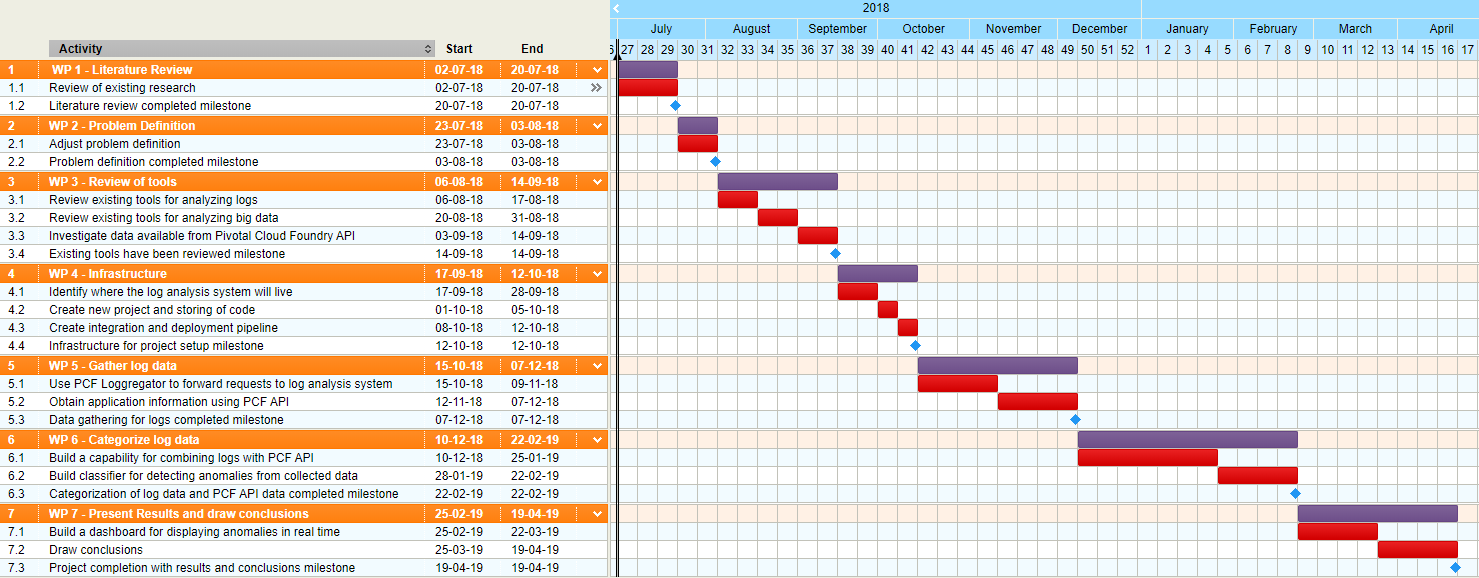
\includegraphics[width=1.0\textwidth]{./figures/gantt.png}
  \caption{gantt}
  \label{fig:gantt}
\end{figure}

\begin{itemize}
  \item \textbf{WP 1} Literature review - 3 weeks - In this work package a literature review on existing approaches to log analysis will be performed.
  
  \item \textbf{WP 2} Problem definition - 2 weeks - Based on the literature review, the challenges of log analysis will be evaluated further. The challenges will produce the definition of key research questions.
  
  \item \textbf{WP 3} Review of tools - 6 weeks - In this work package, available tools for log analysis will be looked at. Additionally, data available in the Pivotal Cloud Foundry API will be investigated.
  
\item \textbf{WP 4} Infrastructure - 4 weeks - This work package involves setting up the infrastructure for the project. Components such as code storage and continuous integration will be acquired and configured in order to enable rapid development. 
  
  \item \textbf{WP 5} Gather log data - 8 weeks - In this work package I will be sourcing logs that will be used for comparative analysis of my service. I will also be setting up Cloud Foundries Loggregator to forward all logs to the analysis service.
  
  \item \textbf{WP 5} Gather log data - 8 weeks - This work package involves sourcing logs that will be used for comparative analysis of my service. Furthermore, setting up Cloud Foundry's Loggregator to forward all logs to the analysis service will be configured.
  
  \item \textbf{WP 6} Categorize log data - 11 weeks - In this work package the delivery of the necessary log analysis algorithms to correctly identify root causes of failures will be performed. A comparison of the benefits of using log analysis with and without PCF API information will be done.
    
  \item \textbf{WP 7} Present Results and draw conclusions - 8 weeks - This work package will deliver a dashboard to display root causes of issues to users. Once complete a report outlining the project observations and conclusions will be written.
\end{itemize}

The milestones that are set to be achieved through the above work packages are as follows.

\begin{enumerate}
  \item Literature review completed
  \item Problem definition completed
  \item Existing tools have been reviewed 
  \item Infrastructure for project setup 
  \item Data gathering for logs completed
  \item Categorization of log data and PCF API data completed
  \item Project completion with results and conclusions
\end{enumerate} % Conclusions and Term 2 work
%\chapter{Ethical Issues}
\lhead{\emph{Ethical Issues}}
If the proposed research directly involves human or live animal subjects, discuss the ethical issues involved and the actions that will be taken to ensure compliance with CIT ethics guidelines and with the CIT Child Protection Policy (if children are involved).
%% ----------------------------------------------------------------
\label{Bibliography}
\bibliographystyle{IEEEtranN}  % Use the "IEEE Transaction" BibTeX style for formatting the Bibliography
\bibliography{Bibliography}  % The references (bibliography) information are stored in the file named "Bibliography.bib"
\lhead{\emph{Bibliography}}  % Change the left side page header to "Bibliography"

%% ----------------------------------------------------------------
% Now begin the Appendices, including them as separate files

\addtocontents{toc}{\vspace{2em}} % Add a gap in the Contents, for aesthetics

\appendix % Cue to tell LaTeX that the following 'chapters' are Appendices

%\chapter{Code Snippets}

Put appendix material in this section e.g. code snippets	% Appendix Title

%\chapter{Wireframe Models} % Appendix Title

%\input{Appendices/AppendixC} % Appendix Title

\addtocontents{toc}{\vspace{2em}}  % Add a gap in the Contents, for aesthetics
\backmatter
\end{document}  % The End
%% ----------------------------------------------------------------